\def\erf{\mathord{\rm erf}}
\def\q#1{q_{\mbox{\scriptsize #1}}}
\def\tp{t_{+}}
\def\tm{t_{-}}
\def\ppart#1{\left[#1\right]_{+}}

\section{Motivation} % (fold)

Flooding resulting from excessive precipitation and surface runoff is a principle cause of significant damage, loss of property, and human suffering throughout the world.  During the GEMT 2010 study group at the Centre de Recerca Matem�tica(UAB) in Barcelona our team was given the task of determining a mathematical model to optimize gate operation along the Ebro River in Spain.
Finding an optimal way to manage these gates is a prominent goal of the CTP projects PREGO (2008ITT00007) and GECOZI (2010CTP00043).

We designed a simple model in which we assumed that the flood wave would maintain its original shape as it propagated downstream.  This simplified model of the situation allowed us to look more closely at the mathematics involved in river flooding and gain some insight on a basic strategy for regulating the flood gates.  In addition to deriving this model for gate regulation we also investigated the costs associated to the situation when $\q{f} > \q{mao}$, i.e. the situation where flooding cannot be avoided.  In this situation it is important to minimize the costs in terms of human suffering and property damage.  We investigate in this paper two methods for approaching the situation where flooding cannot be avoided, there are two methods to consider in this case, Strategy A: opening the gates when $\q{f}$ is achieved, or Strategy B: opening the gates when $\q{mao}$ is achieved, this paper will discuss the analysis of both strategies in detail.  Finally at the conclusion of our analysis we will state some future problems that might be taken up by our group or other researchers with an interest in this problem.

\subsection{States} 

The initial data is the forecasted avenue hydrogram (the graph of
the flow as a function of time) computed from observations at a point
upstream of the control point. Two parameters are relevant: the \emph{maximal
flow} and the \emph{total volume} of the avenue.

We assume that the water height at the control point is a increasing
function of the flow $q$ at that point.

Let us considere three states related to the flow $q$:
\begin{itemize}
\item The \emph{steady state} corresponds to $q<\q{min}$, where $\q{min}$
is the flow that brings the water at the control point high enough
for the gates to open. 
\item A\emph{ typical avenue} state corresponds to $\q{min}<q<\q{mao}$. The
flow $\q{mao}$ is the maximum flow for a recurrent avenue, one that
happens every two or three years. 
\item The \emph{high avenue} state happens when $\q{mao}<q<\q{max}$, where
$\q{max}$ is the flow that makes the water level spill over the floodable
areas. 
\item Finally, when $q>\q{max}$ 
\end{itemize}
For this the following control strategies are defined: 
\begin{itemize}
\item If the maximum forecast flow $\q{i}$ is less than $\q{mao}$, the gates
are not opened. 
\item When $\q{i}>\q{mao}$ and $\q{f}<\q{max}$. In this case the goal is to minimize
the peak discharge after leveling. To compute this, one cuts from the hydrogram an area equivalent
to the capacity of the floodable areas, to get a maxim plateau of
$\q{f}$ flow. 
\end{itemize}



% (end)




\section{First Simple Model} % (fold)

First we will discuss a simple control strategy:
\begin{quote}
	Given a set point $\q{f}$, open the gates completely when the discharge reaches this threshold.
\end{quote}

As a simple first approximation, we ignored the geometry of the river bed and assumed that the flood wave would maintain its shape as it propagated down the river.
We will also assume the height of the river at a given point depends only on the discharge at this point by a increasing function.
In this way we could use height and discharge interchangeably.

Given that opening a gate to a floodplain can reduce the flood by a given volume $W$, we look for the set point $\q{f}$ to
open and close the gate in order to reduce the flood by this area optimally.

Mathematically speaking, we define the discharge of a flood wave at the gate point as $q(t)$ and
choose a refrence interval $[t_0,t_1]$ containing the flood episode.
For simplicity, assume as well that $q$ is unimodal and has a forecast maximum discharge $\q{i}$
expected at time $t_m\in[t_0,t_1]$.
Now define for all $0<y\leq\q{i}$:
\begin{equation}
V(y)=\int_{t_0}^{t_1}\ppart{q(t)-y}\, dt\leq W,
\end{equation}
where $\ppart x =\max\{x,0\}$.

This expression could be
written on the time interval defined by the condition $q(a)=q(b)=y$ with $t_0\leq a\leq t_m\leq t_1\leq b$
using an iterated integral as
\[
V(y)=
\int_{a}^{b}\left(\int_{y}^{q(t)}dq\right)dt.
\]
By inverting the order of the integration, we get
\begin{equation}
V(y)=
\int_{y}^{\q{i}}\left(\int_{\tm(q)}^{\tp(q)}dt\right)dq=
\int_{y}^{\q{i}}(\tp(q)-\tm(q))\, dq,	
\end{equation}
where $\tm(q)$
(respectively $\tp(q)$) is the unique $t<t_{m}$ (respectively
$t>t_{m}$) with $q(t)=q$. Since $V'(y)=\tm(y)-\tp(y)\leq0$,
$V(y)$ is decreasing with $V(\q{i})=0$ and it is easy to find the
unique point $\q{f}$ such that $V(\q{f})=W$ by numerical integration
followed by bisection or inverse interpolation.




\subsection{A numerical experiment}

We tried this idea with a mock floodwave made by adding a Rayleigh function to a constant flow.
(We choose such a function because real floodwaves are typically asymmetrical, see \cite{Lon})
\begin{equation}
q(t) = 1 + 40 \frac{\ppart t}{\sigma^2} e^{-t^2/(2\sigma^2)} 
\end{equation}
with $\sigma=10$ and a goal capacity of $W=22$.
The discharge is sampled between $t=-10$ and $t=100$ for 1000 points (Assuming one hour as time unit, this means roughly a sample each 6 minutes).
The procedure was as follows:
\begin{enumerate}
	\item The maximum discharge $\q i$ is located at point $t_m$ by inspecting the first differences of the sampled data ($M$ data points). This partitions the time samples in two sets: the domains of $\tm$ and $\tp$.
	\item The difference $\tp(q) - \tm(q)$ is approximated by inverse interpolation of $q(t)$ data, for a uniform sampling of $N$ values between the steady flow ($q=1$) and the maximum flow ($q=\q i$).
	\item By cumulative addition we approximate $y\mapsto \int_y^{\q i}(\tp(q) - \tm(q))\,dq$;
    \item Again by inverse interpolation of the above table, we compute $q=\q f$ for $y=W$.
\end{enumerate}
\begin{figure}
\begin{center}
\includegraphics[scale=0.8]{cut}\label{fig:cut}
\end{center}
\caption{\textbf{Left}: $V(q)$ for the test function with the cut volume $W=22.0$
corresponding to $q=\q f$.\textbf{ Right}: The cut volume is the part
of the graph of the test function above $q=\q f$. }
\end{figure}

For $M=1000$ and $N=100$ and $W=22$, we got $\q f\approx 1.70$,  $\tm(\q f)=1.782$ and $\tp(\q f)=22.613$. To check the accuracy of this simple procedure, we compare the integral (which could be computed exactly in this case as $F(t)=t-k(1-e^{-t^2/(2\sigma^2)})$) for $k=40$ and $\sigma=10$ giving
\begin{equation}
\int_{\tm(\q f)}^{\tp(\q f)}q(t)\,dt = F(\tp(\q f)) - F(\tm(\q f)) = 57.09,
\end{equation}
while $W + \q f(\tp(\q f) - \tm(\q f)) = 57.44$.

% (end) Simple model


\section{Heavy Flooding} % (fold)

However, when the flooding is particularly heavy, the capacity of the floodplains maybe insufficient. In this case, even when the peak of the flood is reduced by $W$, it is still higher than $\q{max}$ the levee height, causing floods. In this situation we have two options for controlling the gates, the first strategy is that the gates are opened as soon as the water level reaches $\q{max}$ and the resevoir is filled to capacity, hence reducing the front of the floodwave. This then gives us more time to deal with the flood, e.g. preparing to open more gates downstream (See figure \ref{fig:1}). 
\begin{figure}
\begin{center}
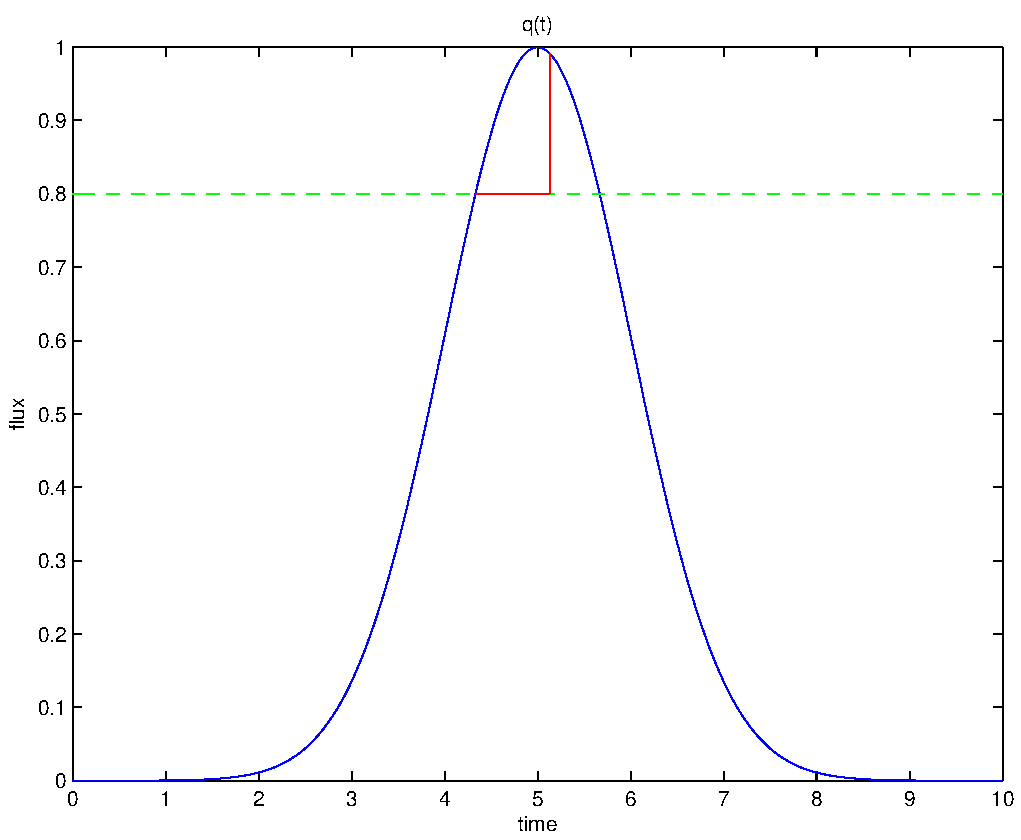
\includegraphics[width=8cm]{fig1}		
\end{center}
\caption{Flux versus time for a peak where flooding is inevitable}
\label{fig:1}
\end{figure}

In the case of flows with multiple flood waves it is always ideal to open the gates at $\q{max}$ instead of $\q{f}$ as it allows some capacity of the floodplain to be reserved for later flood waves. Thus when we have multiple flood waves we will never open the gates before $q = \q{max}$.  
See figure \ref{fig:2} for a situation involving multiple waves and
figure \ref{fig:3} for a case where we can do even better.

\begin{figure}
\begin{center}
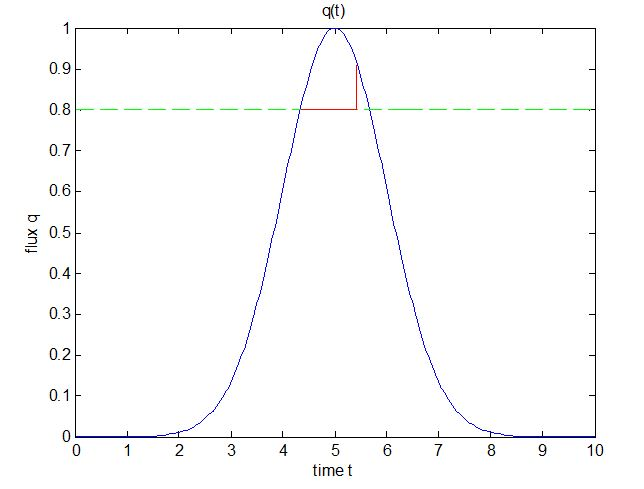
\includegraphics[width=8cm]{fig2}
\end{center}
\caption{Opening the gate at $\q{max}$ allows maximum remaining capacity for the second flood wave.}
\label{fig:2}
\end{figure}



\begin{figure} \centering
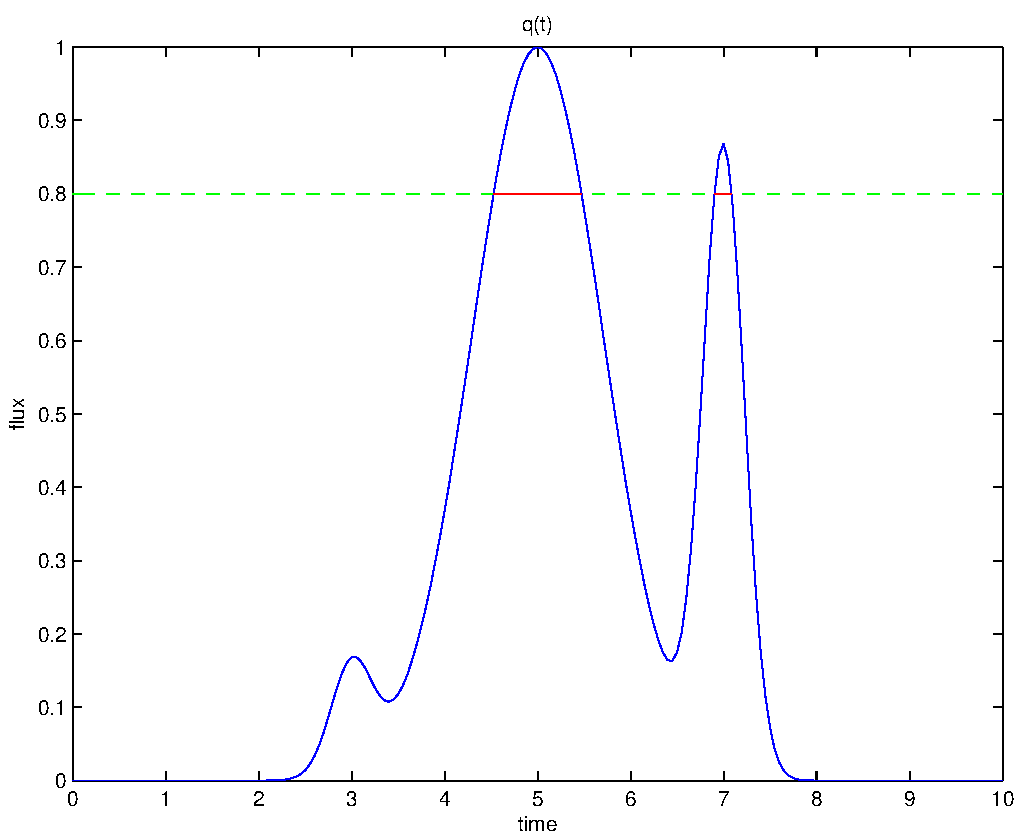
\includegraphics[width=8cm]{fig3}
\caption{Opening the gate at $\q{max}$ allows us to prevent flooding entirely in this case.}
\label{fig:3}
\end{figure}
% (end)

\section{Cost modelling of the main strategies in a flooding} % (fold)
%\subsection*{Main problem: there are two possible strategies}
%The objective of this section is to extract a numerical criteria based on the observations that have been carried out in the previous sections. Note that assuming that a heavy flooding is about to happen we may be able to define two possible strategies to follow.
In this section we assume that a flood that can not be totally prevented is about to happen.
 Recall that a flooding  corresponds to scenario $\q{mao}<\q{f}$ and then, any possible gate opening strategy can avoid that the water level of Ebro surpasses at the analysed point the constructed walls and that floods the surrounding lands. When this happens, the controller of the gate opening must choose when to open the gate in order to reduce as much as it is possible the damage caused by the flooding. In this case, note that two main strategies can be raised: the gate can be either opened when the flow $q$ achieves $\q{mao}$ or it may be opened when $q_f$ is achieved.

The objective of this section is to extract a numerical criteria based on the observations that have been carried out in the previous sections that allows us to choose the best strategy in each possible situation.

As we are going to analyse, each strategy has advantages and drawbacks: 
\begin{itemize}
\item On the one hand, if the gate is opened at $\q{mao}$, the flood is going to be delayed as much as time as possible. However, once the flooding capacity is overpassed, we are not going to have any control of the amount of water that the river carries from this point on. Hence, when the flooding arrives to the most sensitive areas the biggest intensity of the  flood will not be mitigated.
%effects will be unknown.
\begin{figure}\centering
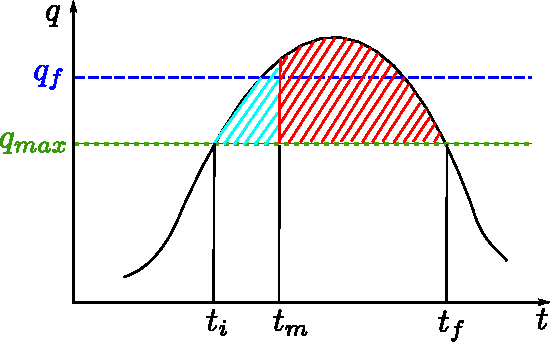
\includegraphics[width=8cm]{basicA}
\caption{Flow diagram for strategy A}
\label{fig:A}
\end{figure} 
Figure \ref{fig:A} shows schematically the inherent idea that defines strategy A. The water coloured in light blue is the amount of water that is able to be drained through the gates. The water coloured in red corresponds to the amount of water that is going to flood the area of interest where we analyse the scenario. Hence, in the presented strategy, once the water overpasses the acceptable level of the river, the door is opened. Then, while the flooding area is able to drain water, the flood is prevented. However, once we are not able to drain more water through the gates, all the remaining flooding water will continue its way, flooding freely the area of interest.
%areas that we wanted to protect as much as we could.

\item On the other hand, the controller of the gate can wait to open it until $q$ achieves $q_f$. Then, the flooding of the sensitive areas starts earlier, whereas the most dangerous peak in the water amount that the flooding carries on is going to be cut out. This way, the main effects of the flooding will be reduced, because the intensity of the flow is going to be lower. However, we are going to let less time to the affected population to leave the affected areas.
\begin{figure}\centering
\includegraphics[width=8cm]{basicB}
\caption{Flow diagram for strategy B}
\label{fig:B}
\end{figure}
Figure \ref{fig:B} shows a water profile of the river channel where strategy B is applied. The colouring scheme is the same than the presented on figure \ref{fig:A}. Hence, figure \ref{fig:B} clearly presents the main drawback and the main advantage of this strategy in front of strategy~A. First, note that the red profile starts earlier than in the previous strategy, and hence, the flooding is not delayed as it happened before. However, the red profile does not get to the high values that strategy A achieved. Hence, strategy B avoids the flood in the peak where it has more intensity.
\end{itemize}

\subsection{Damage cost function}
Accounting for a correct selection of the strategy to follow in each possible scenario, we aim to define a cost 
 function in order to measure the human, economical,etc.\ cost of each strategy. The defined cost function takes on account two main factors:
 \begin{itemize}
 \item the number of affected people depending on the heigh of the water in the flood, and 
 \item the time that the strategy is able to delay the flood.
 \end{itemize}
  %The cost function that we are going to consider is defined as equation \ref{cost} shows. 
%  The cost that we are assuming from an initial time $t_i$ to a certain time $t$ is given by:

%Assuming that the flooding starts at a given time $t_i$ and that it lasts until a certain time $t$, the proposed cost function is
Assuming that the flooding starts at a given time $t_0$, the proposed cost function of the flood at a certain time $t$ is
\begin{equation}
C(t)=\int_{t_0}^{t}\frac{\rho(h(q(t)))}{t}dt,
\label{cost}
\end{equation}
where $\rho$ is the density of population that lives below a certain heigh $h$. Note that the heigh of the flooding is a function of of $q$ (the height that the flooding affects to depends on $q$), and that both $q$ and $h$ are known in any possible scenario. We have divided the density by $t$ in order to ``decrease the cost'' when increasing the time, since we want to minimize the effects of the flood but we also want to penalise the time that a strategy  gives to the population to leave the affected zone. 

Note that in this cost function definition, it can be decided if more importance is given to the amount of affected people, or to the delaying of the flooding. For instance, if we want to give more importance to the delay of the flood we can change the modelling cost and use some other $t^r$, $r>1$, penalising then an strategy that does not let time enough to the population to evacuate. Analogously, if we choose not to involve the delaying time in the cost penalization, we can also take $r=0$.

\subsection{Finding the strategy that minimizes the cost function}
Given an scenario, we do know all the variables that are involved in the definition of the cost function \eqref{cost}. Hence, in order to execute the better strategy, we only require to compute the integral \eqref{cost} and take the strategy with a lower cost.
%We want then to compute the cost function for each one of the two main strategies to follow in a flooding scenario. Hence, 
 The most valid strategy is the one that results in the minimum cost at the ending time of the flood, $t_1$.
 
 However, it may be interesting to be able to know a priori bounds about the possible cost of each situation. Hence, we could have information before the flooding occurs about how each strategy behaves and, for example, we could be able to fix a default strategy that is known to be safer through the a priori bounds. Furthermore, if we ever are able to find lower and upper bounds for both strategies we may find interesting conclusions about the procedure to follow when a flood occurs.

\begin{description}
\item[Strategy A:] Opening the gates when $\q{mao}$ is achieved.

\noindent With strategy A we find that despite reaching higher flow values, the time in which $\q{mao}$ is surpassed is delayed, and thus there are no costs  for a longer time than in strategy A. However, we are just able to delay the flow until a known time $t_m$, where the auxiliary flooding area is full and we can not take more water from the river. Thus, the cost of strategy A is
\begin{eqnarray*}
C(t_1)=\int_{t_0}^{t_1}\frac{\rho(h(q(t)))}{t}dt=\int_{t_m}^{t_1}\frac{\rho(h(q(t)))}{t}dt,
\end{eqnarray*}
where we must recall that all the data required in the integral is known, and thus, in a particular case it is straight forward to compute the cost.
\newline
Hence,
\begin{equation}
C_A=\int_{t_m}^{t_1}\frac{\rho(h(q(t)))}{t}dt
\label{costA}
\end{equation}
is the cost of strategy A.

Note that an upper bound of this expression can be found:
\begin{eqnarray*}
C_A&=&\int_{t_m}^{t_1}\frac{\rho(h(q(t)))}{t}dt 
\leq\int_{t_m}^{t_1}\frac{\rho_*}{t}dt \\
&=& \rho_* \ln\left(\frac{t_1}{t_m}\right) =: \hat{C}_A,
\end{eqnarray*}
where $\rho_*=\rho(h(q_*))$, being $q_*=\max_{t\in(t_m,t_1)}q(t)$, the peak value of $q$. Recall that this bound may be slightly coarse, but it is useful in the sense that if the cost that the bound assigns is acceptable compared to B, then the strategy is valid for our purposes.

\item[Strategy B:] Opening the gates when $\q{f}$ is achieved.

\noindent
For this strategy we can easily find an accurate upper bound for its cost. Note that except at the beginning and at the end of the flow diagram, the flow that is flooding the area of interest is know, since we cut it using the gates at $q_f$ value. Hence, we control that $q(t)=q_f$ in all the diagram except in a small region, where $q(t)\leq q_f\ \forall t$. Thus,
\begin{eqnarray*}
C(t_1)&=&\int_{t_0}^{t_1}\frac{\rho(h(q(t)))}{t}dt \leq \int_{t_0}^{t_1}\frac{\rho(h(q_f))}{t}dt\\
&=&\int_{t_0}^{t_1}\frac{\rho_{q_f}}{t}dt=\rho_{q_f} \ln\left(\frac{t_1}{t_0}\right),
\end{eqnarray*}
where we have denoted by ${\rho_{q_f}}$ the density of population that lives below $h(q_f)$.
\newline
Thus,
\begin{equation}
C_B=\int_{t_0}^{t_1}\frac{\rho(h(q(t)))}{t}dt
\label{costB}
\end{equation}
is the cost of strategy B, and it can be bounded as
\begin{equation}
C_B \leq \rho_{\q{f}}\ln\left(\frac{t_1}{t_0}\right) =: \hat{C}_B,
\label{CB}
\end{equation} 
where $\rho_{q_f},\ t_0 \text{ and } t_1$ are all known.

%Recall that this is a useful bound, since it tells us a priori that the cost of this strategy is always going to be under $\rho_q\cdot\ln(\frac{t_f}{t_i})$. % If we assume that this is a feasible cost, we may be able always use this strategy
\end{description}

Depending on the scenario that is placed we can compute both $C_A$ and $C_B$ and have a reference of which one of the strategies will bring up more advantages. The bounds are simplified expressions that require less data and give useful information, since they tell the limit of the cost that the strategy may result in. 

However, note that judging just by the a priori found bounds of both strategies no conclusions can be drawn about if there is one strategy that is always better than the other one just judging by either the affected population or the maximum flood capacity. No a priori conclusions can be extracted from the comparison $\hat{C}_A \leq \hat{C}_B$.

Summarizing, we first have been able to develop two main strategies to deal with a flood. Moreover, we have defined a cost function that can be used as a key to choose the ideal strategy to select in each scenario. Two upper bounds of the cost of both strategies have been extracted. However, no conclusions about the selection of the best strategy can be drawn just by judging the a priori bounds.

% (end)

\section{Conclusion and Further Work} % (fold)

In this paper we have stated an algorithm for determining the opening and closing times of a single flood gate.  In addition we have studied how cost functions can be used to minimize damage and hardship caused by flooding in highly populated areas along the Ebro River.

We propose that in future research studies the case of gate control is considered more closely, perhaps in conjunction with the idea of minimizing costs in the case that flooding cannot be avoided.  The most important extension of our ideas is to work with multiple gates and multiple flood waves.  This case will be more complex but also will more closely impact actual implementation of gate control along the Ebro River.  By assigning a cost to the flooding of particular floodplains it will be possible to obtain the minimum amount of damage in the case that we cannot prevent a flood with the gate control scheme.  
% (end)